% !TEX root = C:/Users/piyus/knowledge/Project_Specific_Knowledge/public/fm_radio/stages/HF_amp/HF_amp.tex
\documentclass[12pt, letterpaper]{article}

\usepackage{hyperref}
\usepackage{graphicx}
\graphicspath{ {C:/Users/piyus/knowledge/Project_Specific_Knowledge/public/fm_radio/stages/HF_amp/pictures} }

\title{High Frequency Amplifier Notes}
\author{Piyush Sud}
\date{9/30/2024}
\begin{document}
\maketitle

\pagebreak

\section{High Level Design}

For the high frequency amplifier, we need:

\begin{itemize}
    \item a large bandwidth (at least 200 MHz)
    \item a high gain
    \item large SNR
\end{itemize}

\noindent The MAR8ASM+ works for this application. It has:

\begin{itemize}
    \item a large bandwidth (25 dB of gain at 1 GHz)
    \item a high gain (31.5 dB at 100 MHz)
    \item large SNR (It gives the figure 3.1 dB at 1 GHz. Assuming this is thermal noise, it is not frequency dependent so this would be the same as the noise at 100 MHz. This is a decently low value.)
    \item Added benefit - the amplifier is internally matched to 50 ohms.
\end{itemize}

\section{Detailed Design}

Using the recommended application circuit:
\begin{figure} [h]
    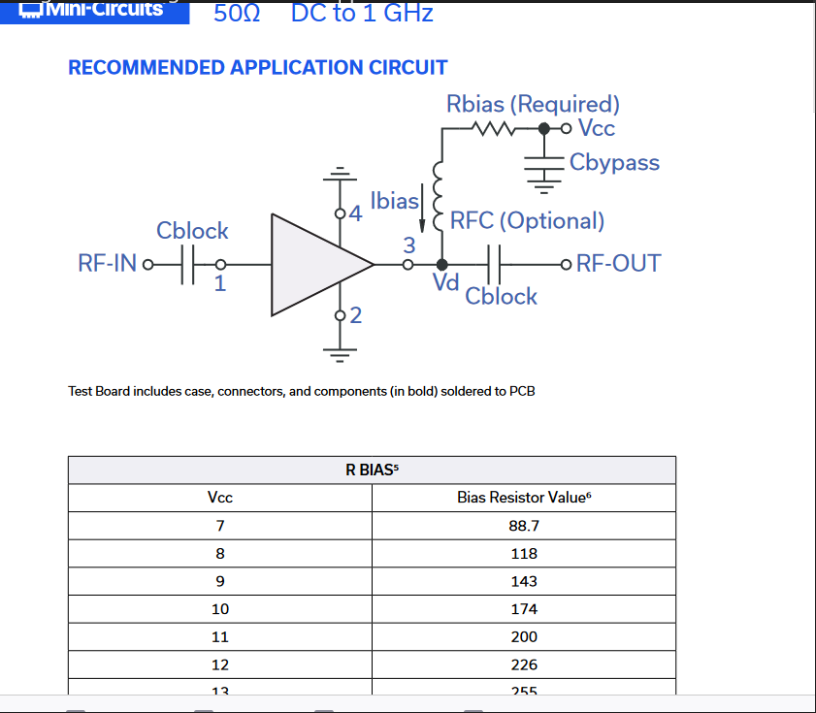
\includegraphics[width=\textwidth]{rec_app_circuit}
\end{figure}

\begin{itemize}
    \item Assuming that Vd = 3.7V (since that is the supply voltage listed on the datasheet), Rbias dissipates \(\frac{V^2}{R} = \frac{(12-3.7)^2}{226} = 0.30482300885 W\). This means we can't choose a regular 1/4 watt or 1/10 watt resistor. Choosing the CRCW2512226RFKEG 1W resistor as a FOS of ~3. 
    \item For Cblock, we want it to block any signal frequencies below 88 MHz. 
    \item Let's set it to 1uF, which would give us an impedance of \(\frac{1}{2\pi j (100*10^6) (1*10^{-6})} -0.0628j \) at 100 MHz and \(\frac{1}{2\pi j (100) (1*10^{-6})} = 62.8k\) ohms at 100 Hz.
    \item Unfortunately, this won't work because I couldn't find any 1 uF capacitors online that would have a self-resonant freq. above 100 MHz.
    \item However, I did find a 0.1 uF broadband capacitor: \url{https://www.digikey.com/en/products/detail/kyocera-avx/530L104KT16T/6570911?s=N4IgTCBcDaIKwGYAMAZABAYwIYAcsYEsAXAewCcQBdAXyA}
    \item It doesn't have a SPICE model, but it does have low insertion loss through 18 GHz, so it should be fine.
    \item What about the self-resonant frequency? According to perplexity, it seems like certain broadband capacitors can damp their resonance or use other advanced techniques to have a low insertion loss throughout the desired frequency range, despite their SRF being in the desired frequency range. Therefore, I am just going to use an ideal capacitor in LTSPICE, not worrying about the SRF.
    \item How much group delay is too much?
    \item From a quick google search, For FM radio, the baseband ranges from 50 Hz to 15 kHz. For 15 kHz, this corresponds to a period of 66 us. Since the group delay for the amplifier is in the ns range, I don't think this is a problem.
    \item As for the MAR8ASM+, I was able to find an s-parameter model which I converted to LTSPICE using S2Spice.
\end{itemize}

\section{Results}
Here is the simulation of the amplifier, with the step like function being the group delay:
\begin{figure}[h]
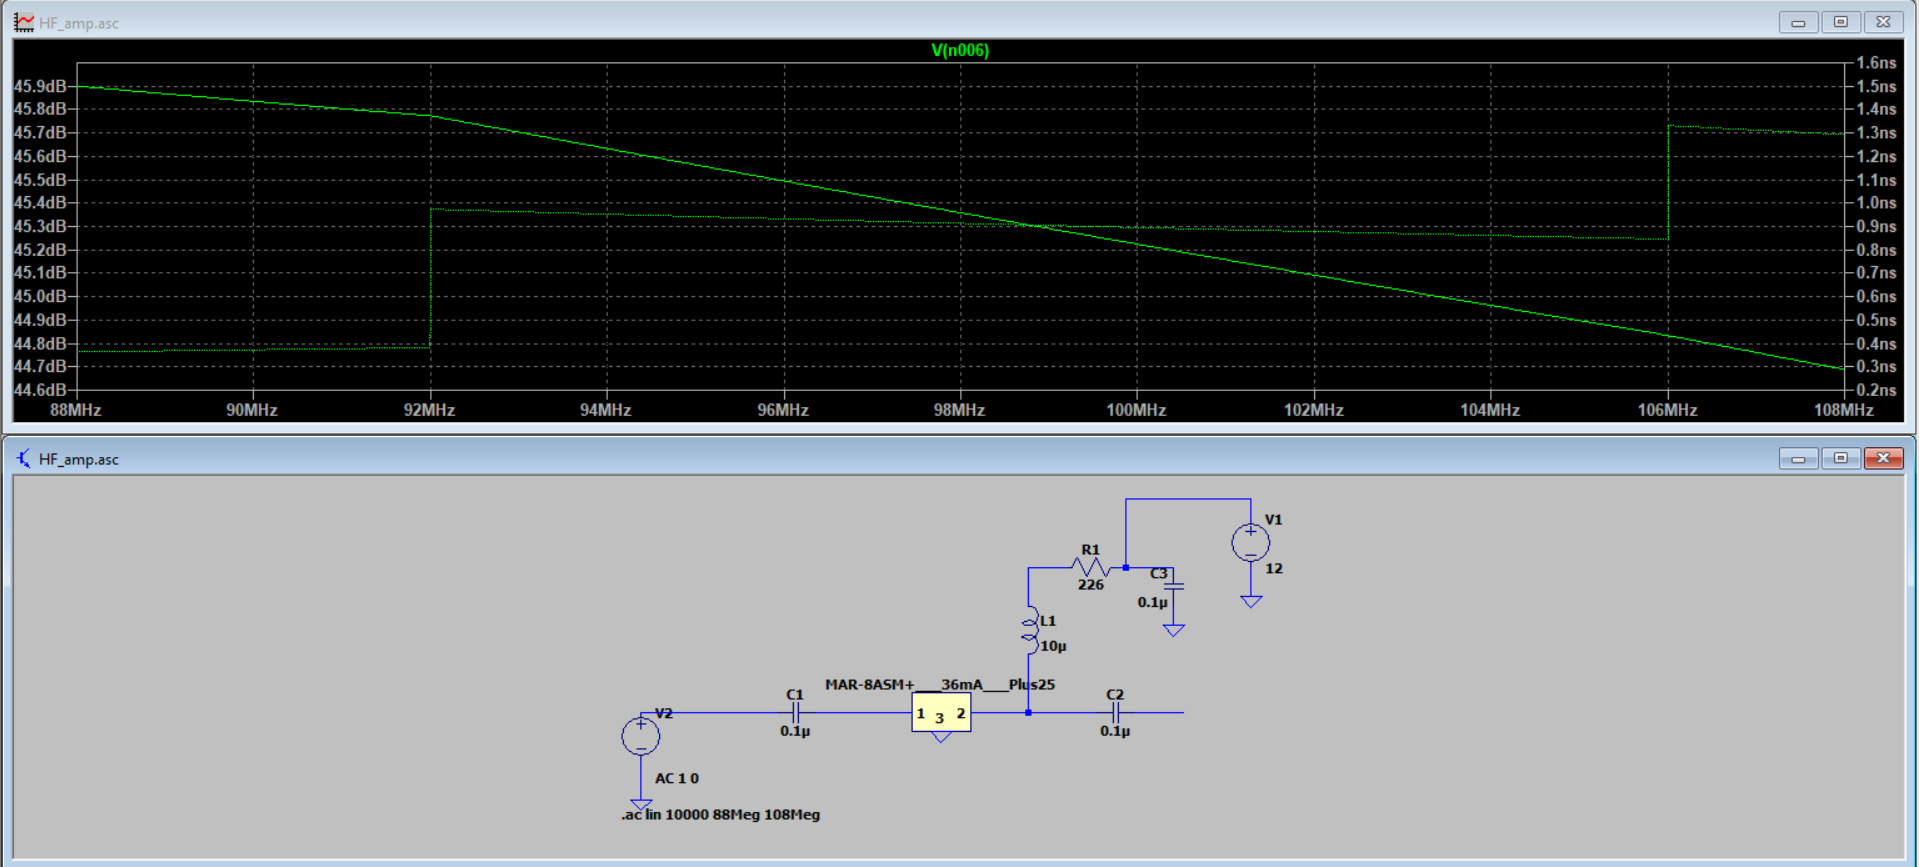
\includegraphics[width=\textwidth]{group_delay}
\end{figure}


\end{document}